\documentclass[11pt]{article}
\usepackage[margin=0.7in]{geometry}
\usepackage{multirow}
\usepackage {graphicx}
\usepackage[utf8x]{inputenc} % указать кодировку русского текста
\usepackage[russian]{babel} % указать, что язык текста - русский
\usepackage{fancyhdr}
\pagestyle{fancy}

\begin{document}

\begin{titlepage}

\begin{center}
%\vspace*{1cm}
\large\textbf{Московский Физико-Технический Институт}\\
\large\textbf{(государственный университет)}
\vfill
\line(1,0){430}\\[1mm]
\huge\textbf{Эффект Холла в полупроводниках}\\
\line(1,0){430}\\[1mm]
\vfill
\large Сибгатуллин Булат, ФРКТ\\
\end{center}

\end{titlepage}
\fancyhead[L] {Работа 2.3.1}
\noindent \textbf{Цель работы:} \\
\indent измерение подвижности и концентрации носителей заряда в полупроводниках\\
\noindent \textbf{В работе используются:} \\
\indent электромагнит с регулируемым источником питания; вольтметр; амперметр; миллиапмперметр; милливеберметр; источник питания (1,5 В), образцы легированного германия.

\section*{Описание работы}

\begin{figure}[h!]
\centering
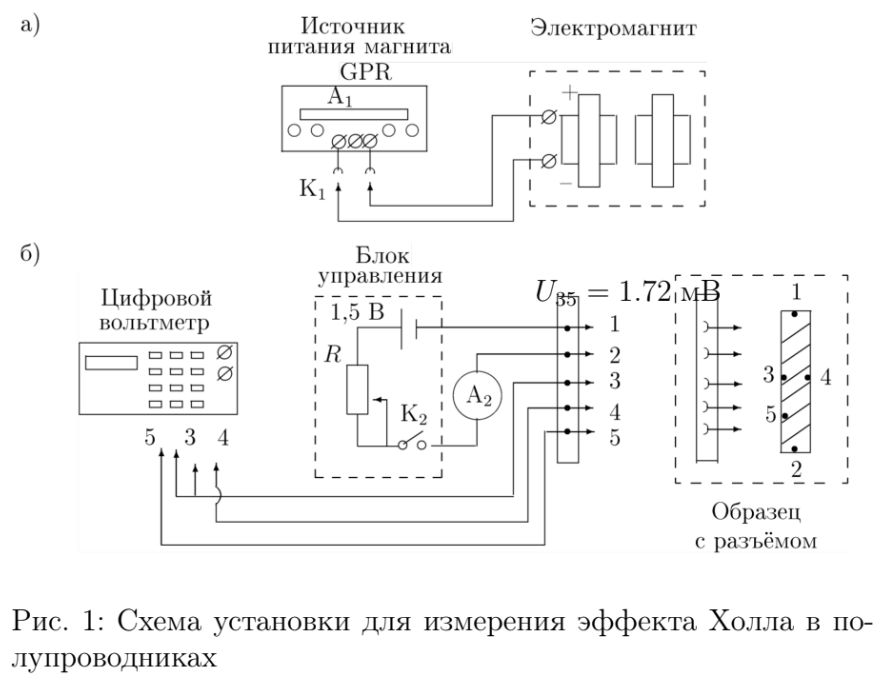
\includegraphics[scale=1]{image1.png}
\label{fig:Image1}
\end{figure}

Электрическая схема установки представлена на рисунке 1. В зазоре электромагнита создается постоянное магнитное поле. Его ток питания измеряется амперметром $A_1$. 

Прямоугольный образец из легированного германия смонтированный в специальном держателе (рис. 1б), подключается к источнику питания. При замыкании ключа вдоль длинной стороны образца начинает течь ток.

В образце помещенном в зазор электромагнита, между контактами 3 и  4 возникает разность потенциалов $U_{34}$, которая измеряется с помощью вольтметра $V$.

Так как контакты 3 и 4 могут лежать не на одной эквипотенциали стоит измерить напряжение в системе без магнитного поля $U_0$ и считать итоговое напряжение по формуле:

\[U_\perp = U_{34} - U_0\]

\newpage

\section*{Ход работы}\

Измерим калибровочную прямую электромагнита - зависимость между индукцией \textit{В} магнитного поля в его зазоре и током $I_M$ через обмотки магнита. Данные занесем в таблицу. Значение индукции можем получить по формуле:

\begin{equation}
B = \frac{\Phi}{SN},
\end{equation}

где $SN = 75$ $\textit{см}^2 \cdot \textit{витков}$.

\begin{figure}[h!]
\centering
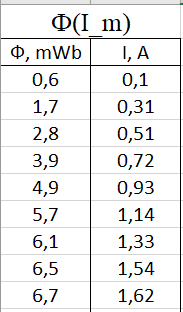
\includegraphics[scale=1]{table1.png}
\label{fig:Image1}
\end{figure}

\vspace{0.5cm}

По получившимся данным построим график $B(I_M)$:

\begin{figure}[h!]
\centering
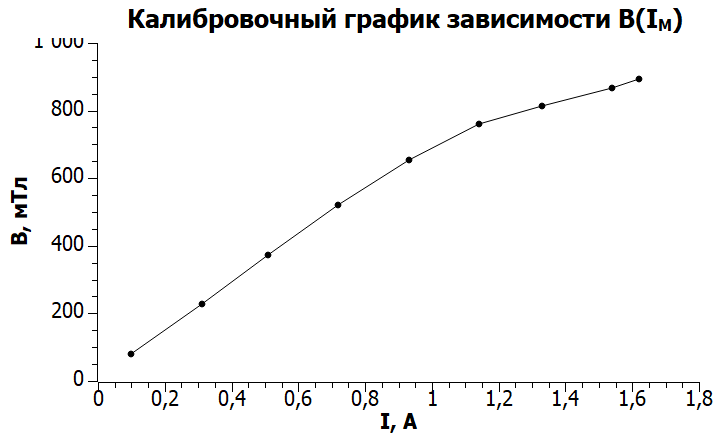
\includegraphics[scale=1]{Graph2.png}
\label{fig:Image1}
\end{figure}

\vspace{0.5cm}

Проведем измерения ЭДС Холла, сняв зависимость напряжения $U_{34}$ от тока электромагнита $I_M$, при фиксированном токе через образец, для токов в диапазоне 0,3 - 1 \textit{мА}. Данные занесем в таблицу. Для значение тока через образец равного 1 \textit{мА} также проведем измерения при обратном направлении магнитного поля.

\begin{figure}[h!]
\centering
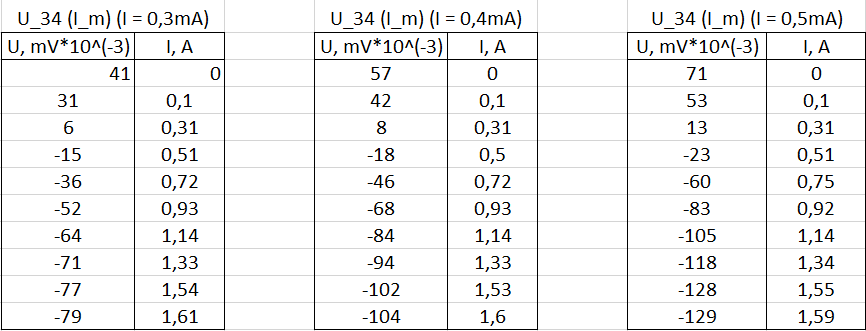
\includegraphics[scale=1]{table2.png}
\label{fig:Image1}
\end{figure}

\begin{figure}[h!]
\centering
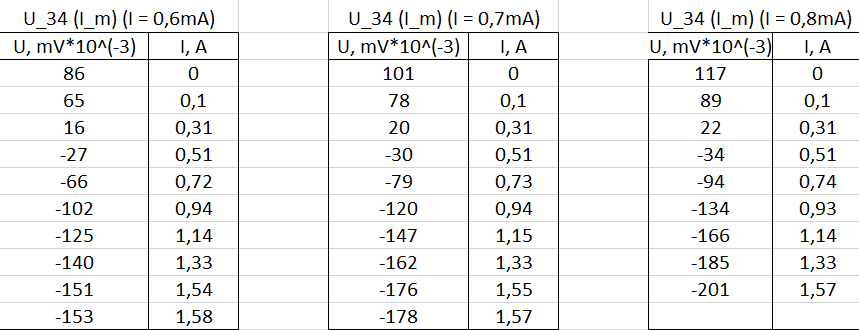
\includegraphics[scale=1]{table3.png}
\label{fig:Image1}
\end{figure}

\begin{figure}[h!]
\centering
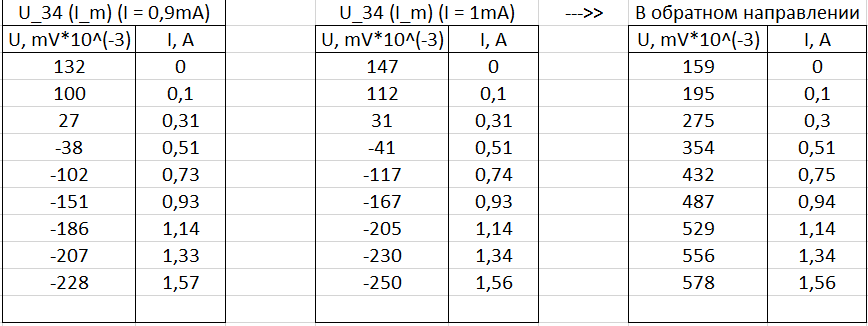
\includegraphics[scale=1]{table4.png}
\label{fig:Image1}
\end{figure}

\vspace{0.5cm}

Для получившихся данных построим на одном листе семейство характеристик $U_{\perp}(B)$.

\begin{figure}[h!]
\centering
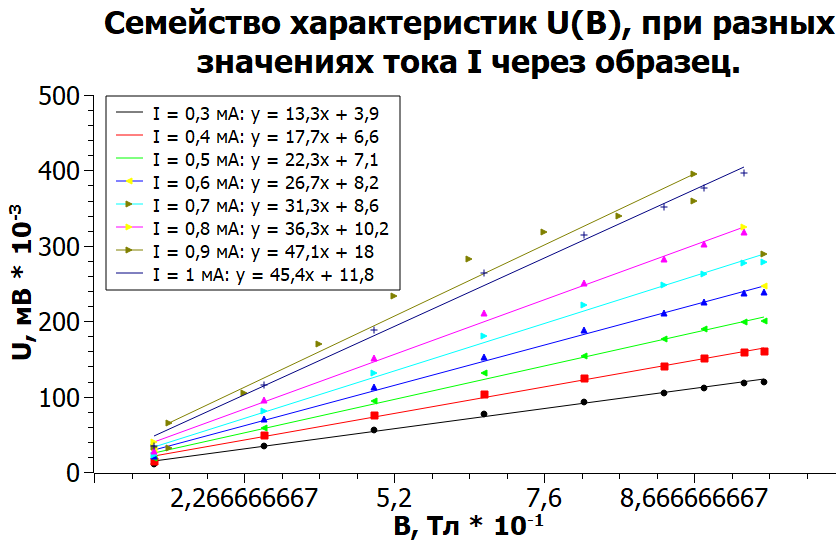
\includegraphics[scale=1]{Graph1.png}
\label{fig:Image1}
\end{figure}

\vspace{0.5cm}

По значениям угловых коэффициентов \textit{k} полученных прямых построим график \textit{k(I)}.

\begin{figure}[h!]
\centering
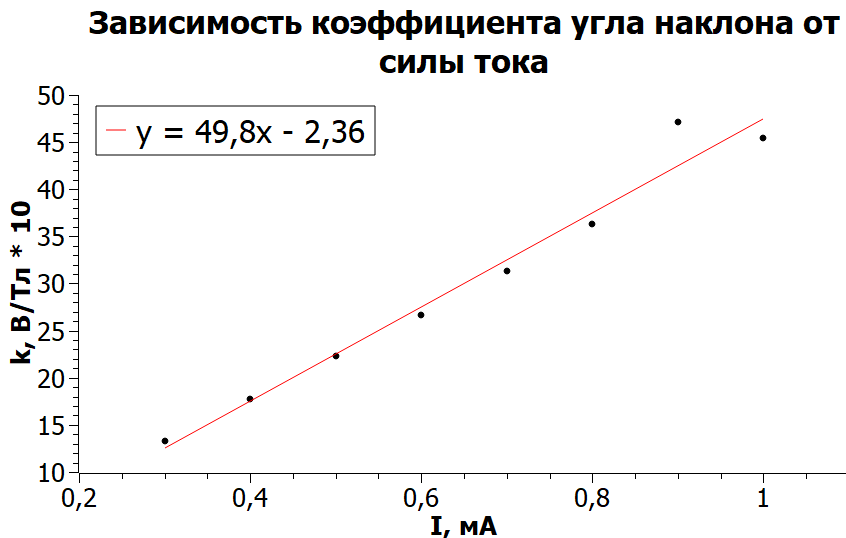
\includegraphics[scale=1]{Graph3.png}
\label{fig:Image1}
\end{figure}

По значению углового коэффициента получившейся прямой $k = 49,79 \pm 3,44$  определим величину постоянной Холла $R_H$ по формуле:

\[R_H = k \cdot a,\]

где $a = 2,2$ \textit{мм}. Тогда в итоге получаем:

\[R_H = (1096 \pm 76) \frac{\textit{м}^3}{\textit{А}\cdot\textit{с}}\]

\vspace{0.5cm}

Определим концентрацию носителей заряда:

\[n = \frac{1}{R_H \cdot e} = (5,68 \pm 0,39) \cdot 10^{21} \frac{1}{\textit{м}^3}\]

\vspace{0.5cm}

Измерим падение напряжения на контактах 3 и 5, $U_{35} = 2,476$ \textit{мВ} при значении тока через образец $I = 1$ \textit{мА}. Параметры образца: $L = 6$ \textit{мм}, $L = 7$ \textit{мм}. Рассчитаем удельную проводимость:

\[\sigma_0 = \frac{I \cdot L}{U_{35} \cdot a \cdot l} = 157 \pm 5 \quad \frac{1}{\textit{Ом}\cdot\textit{м}}\]

Вычислим подвижность $\mu$ носителей тока:

\[\mu = \frac{\sigma}{en} = 0,173 \pm 0,013 \quad \frac{\textit{м}^2}{\textit{В}\cdot\textit{с}}\]

\section*{Вывод}\

Определили постоянную Холла для Германия и оценили удельную проводимость и подвижность носителей тока для нашего образца. Также определили, что в нашем случае реализуется проводимость дырочного типа.

\end{document}